\section{Viscous API Implementation}
We have implemented and tested Viscous protocol using C++ language in Linux kernel environment with \texttt{pthread}. We have made the Viscous implementation open-source, which is available at \url{https://github.com/abhimp/Viscous}. Complete API details and additional implementation details are available at \url{https://abhimp.github.io/Viscous/}.  
%The implementation details of Viscous is discussed next. 

%We have performed most of the experiment in network emulator Mininet and real network using raspberry pis. 

%Before we go deep into implementation, we will discuss the packet structure being used in our implementation.

\subsection{Viscous Packet Structure}
In Fig.~\ref{fig:packet_format}, we have depicted the packet structure used in our implementation. 
Each packet is divided into three parts -- a) mandatory header, b) variable length optional headers for additional information, and c) data region. The $28$ byte mandatory header has all the common fields required for the communication. The details of the mandatory fields are as follows. 
%
\begin{figure}[!t]
    \centering
    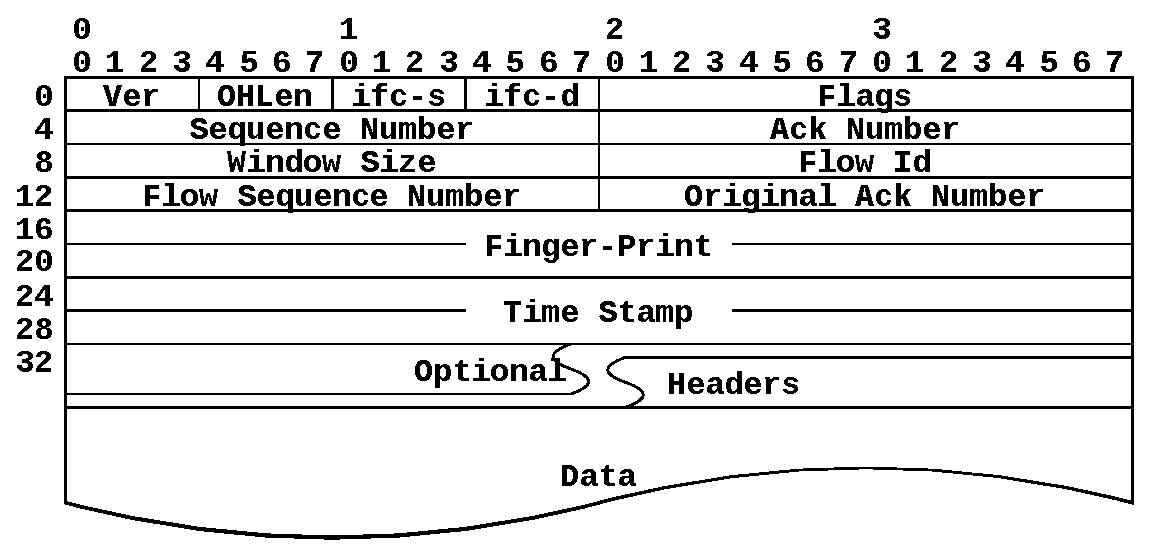
\includegraphics[width=0.85\linewidth]{img/Packet_format.eps}
    %\framebox[0.9\linewidth]{\input{img/Packet_format.tex}}
    \caption{Viscous packet header structure}
    \label{fig:packet_format}
\end{figure}
%\subsubsection{Mandatory header}
%Every packet starts with 28 bytes mandatory headers. It several fields. These fields are:
%\begin{itemize}
 
\noindent \textbf{Ver}: $4$ bits protocol version number. 
  %The current version is 1.
    
\noindent  \textbf{Optional Header Length(OHLen)}: We have optional headers of different sizes. This field helps decoder to understand how many optional headers need to be read before data section can be reached.
    
\noindent \textbf{ifc\_s}: 4 bit application defined source interface ID.
 
\noindent  \textbf{ifc\_d}: 4 bit application defined destination interface ID.

\hspace{3pt} Each application can use the device and list down the interface ids available. We assume that a device cannot have more than 15 interfaces. Interface ids start with 1. Interface id $0$ (zero) means it is not a valid interface. In our implementation, we use a pair of local and remote interface id as channel identifier. So, our implementation can support at most ($15\times15$) $225$ channels.
    
\noindent  \textbf{Flags}: We have used a set of boolean flags. It is similar to TCP. However Viscous need more flags as it is significantly different from TCP.
    
\noindent  \textbf{Sequence Number}:  Unlike TCP, the sequence number in Viscous is used to identify a packet rather than the byte stream. We use packet based sequence number because of two reasons -- a) packets are not created by channel handler; and b) as we multiplex multiple flows, it is easier to track a packet from a flow than a byte stream from a flow. Sequence numbers are used by channel handler to provide reliable communication between two applications. It can be noted that two channels can have same sequence number.
    
\noindent  \textbf{ACK Number}: It is cumulative acknowledgment number like TCP acknowledgment number. It denotes that the receiver has received contiguous packet up to this sequence number and it did not receive next packet until the time it was sent from the receiver.
    
\noindent \textbf{Window Size}: Receiver's advertise window. Channel does not use this window size. It is for flow handler.
    
\noindent  \textbf{Fingerprint}: It is Viscous client's unique ID generated by the server. Every packet includes this field except the initial synchronization packet for connection establishment. In Viscous, packets are discarded if this field is zero or if there is no connection matching this fingerprint (i.e. invalid fingerprint).
    
\noindent  \textbf{Flow ID}: Flow ID is an important field in a Viscous packet, which is used by the multiplexer to identify appropriate flow and to forward received packet accordingly.
    
\noindent  \textbf{Flow Sequence Number}: Each flow has its flow sequence number independent of the sequence number used by the channel. It requires at the flow layer to reorder the packets at the receiver side. We use packet based flow sequence number in Viscous, similar to the sequence number field.
    
\noindent  \textbf{Original ACK Number}: Viscous uses selective acknowledgment mechanism. When the receiver receives an out of order packet, it is supposed to send duplicate acknowledgment packet acknowledging the last conscious packet received. The receiver puts the original sequence number of the packet, which triggers the duplicate acknowledgment. This field gives sender an indication about packets received at the receiver side. So, the sender does not resend them again. It helps Viscous in reducing overall retransmission.
    
%    \item \textbf{Padding}: It is not a field.
    
\noindent  \textbf{Sent time-stamp}: When a sender sends a data packet, it includes the current Unix timestamp in microseconds ($\mu{s}$). When a receiver receives a data packets, it includes this timestamp with the ACK packet. It helps the sender in measuring the RTT more accurately.

\subsection{Modules and Layers in Viscous}
Viscous follows a modular architecture as shown in Fig.~\ref{fig:ModularDiagram}. The various modules in Viscous are as follows. 

\subsubsection{Application}
An application is the users' application that uses Viscous library. 


\subsubsection{Flow Handler}
In Viscous, an application directly sends data to this module and receives from it. Flow handler packetizes the raw data from the application and sends packets to the lower layer for further processing. It does not need to store any outgoing packets, as the channel layer ensures the reliability. It only keeps track of the packets that it sends, to control the flow rate. Viscous uses a sliding window based flow control mechanism based on the receiver advertised window size.
The flow handler also reorders the out of order packets that it receives from the lower layer. There is a receive buffer that stores all the out of order packets. This buffer is an array of packets. The first index of this packet array point to the next expected packet sequence. Whenever the flow handler receives one or more contiguous packets from the expected sequence, it delivers the data from those flows to the application. In Viscous, there is one independent flow handler instance for each of the flows.

\subsubsection{Multiplexer}
The multiplexer is responsible for multiplexing the outgoing packets from multiple flows and forwarding them to the packet scheduler. It is also responsible for demultiplexing incoming packets and forwarding them to appropriate flow handler. 

\begin{figure}[!t]
	\centering
	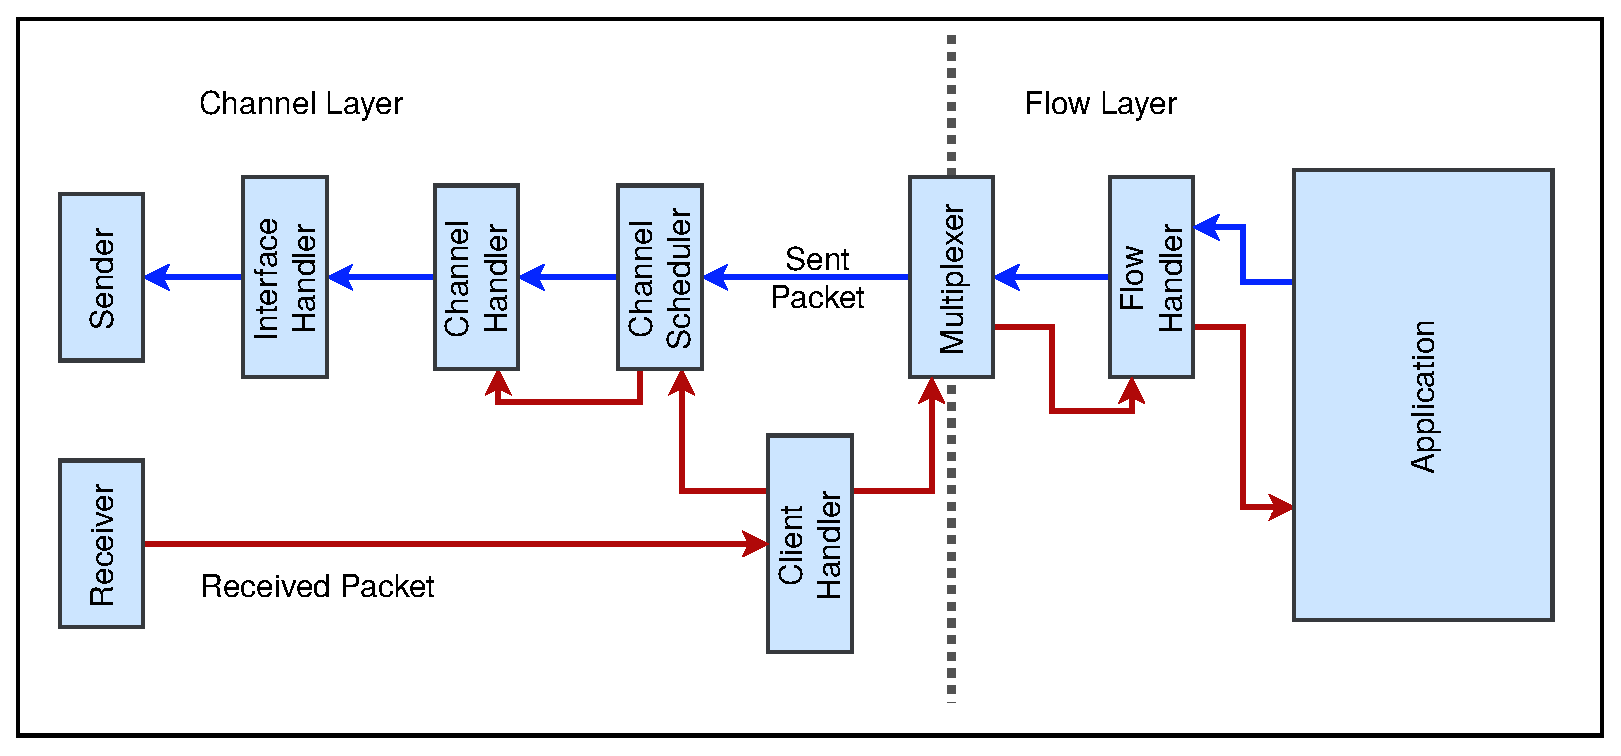
\includegraphics[width=.9\linewidth]{img/ModularDiagram}
	\caption{Internal packet and data flow diagram}
	\label{fig:ModularDiagram}
\end{figure}


\subsubsection{Client Handler}
Client handler is the manager of Viscous protocol API. 
For incoming packets, it checks the packet validity using the fingerprint generated during the connection establishment. 
After validation, it forwards each incoming packet to the {\em Channel Handler} via {\em Channel Scheduler} for further handling and processing for congestion control algorithm. 

\subsubsection{Channel Scheduler}
It schedules the outgoing packets to one of the channels. As mentioned earlier, we use \texttt{ACK} driven channel scheduling. Whenever a channel is ready to send packets, it asks the {\em Channel Scheduler} for new packets to be sent. A smart scheduler can decide which packet to be sent through a channel based on its algorithm to achieve high throughput with lower latency.


\subsubsection{Channel Handler}
Channel handler is responsible for reliable communication and congestion control in the network. We have discussed the congestion control algorithm in detail in section \ref{section:congestion_control}.

%In the Viscous implementation, we use the TCP New Reno congestion control~\cite{RFC2582} algorithm with the following modifications. In Viscous, the channel handler handles packets, not TCP like byte streams. So, we use packet based sequence number because it is easier to track a packet from a flow than a byte stream from a flow when we multiplex multiple flows. Further, in the Viscous congestion control, each \texttt{ACK} contains the sequence number of the packet for which this acknowledgment is triggered. This gives a similar effect as TCP selective acknowledgment (\texttt{SACK})~\cite{RFC2018} mechanism. Further, as flows are multiplexed, we have modified the fast recovery phase describe in RFC2581~\cite{RFC2582} with \texttt{SACK} modifications. After receiving the first partial new \texttt{ACK}, the channel handler sends all the unacknowledged (via \texttt{SACK} or original \texttt{ACK} in the packet header) packets up to the received acknowledgment number for each duplicate \texttt{ACK}. This modification reduces retransmissions due to timeout events when a series of packets get lost in the network.

\subsection{Mobility}
In our implementation, we have implemented Individual mobility for both the client and the server side. We consider the changes in network interface as external event. It was difficult to capture those events automatically from the application itself. So, for now we use a hack to catch those event. A Viscous application creates a {\it named fifo} in a predefined path (configurable via environment variable) to interact with other processes. There is a tool name NetworkManager available in most linux system can successfully capture all kind of events related to network interface in a  device. It also run various {\tt bash} script from the {\tt /etc/network} directory. We take advantage of this tool and put two scripts in the directory. One script runs when some network interface gets connected and another script runs whem a interface gets disconnected. These script passes this information to all the Viscous applications running in the device via the {\it name fifo}. This is a hack and we are working on the more generic way to capture the events.

%In our implementation, we have implemented Individual mobility for both the client and server side. We consider change in network interface as external event. To generate this event, we take help from NetworkManager tool available in most of the Linux distribution. Every time a interface gets connected or disconnected, NetworkManager run different script from {\tt /etc/network} directory. We take advantage of this behavior. We put few extra scripts there to pass those events to Viscous application via {\it named fifo} created by the application in predefined path. In the implementation, viscous library creates a {\it named fifo} in a predefined path and try read information in that fifo.

